\documentclass[12pt,a4paper]{report}

% ---------- Langue et encodage ----------
\usepackage[utf8]{inputenc}
\usepackage[T1]{fontenc}
\usepackage[french,provide=*]{babel}

% ---------- Mise en page ----------
\usepackage[margin=2.5cm]{geometry}
\usepackage{setspace}
\onehalfspacing
\usepackage{fancyhdr}
\setlength{\headheight}{15pt}
\pagestyle{fancy}
\fancyhf{}
\renewcommand{\headrulewidth}{0.4pt}
\fancyhead[L]{\nouppercase{\leftmark}}
\fancyhead[R]{\thepage}
\renewcommand{\chaptermark}[1]{\markboth{\thechapter.\ #1}{}}

% ---------- Tableaux, figures, graphiques ----------
\usepackage{graphicx}
\usepackage{booktabs}
\usepackage{longtable}
\usepackage{array}
\usepackage{multirow}
\usepackage{makecell}
\usepackage{caption}
\usepackage{float}
\usepackage{pgfplots}
\pgfplotsset{compat=1.18}
\usepackage{tikz}

% ---------- Mathématiques ----------
\usepackage{amsmath,amssymb}

% ---------- Couleurs ----------
\usepackage{xcolor}
\definecolor{itieblue}{RGB}{0,61,107}
\definecolor{itiegold}{RGB}{196,154,49}

% ---------- Liens et bibliographie ----------
\usepackage{hyperref}
\hypersetup{
  colorlinks=true,
  linkcolor=itieblue,
  citecolor=itieblue,
  urlcolor=itieblue,
  pdftitle={Impact du régime fiscal minier sur les recettes publiques au Sénégal},
  pdfauthor={Stagiaire ITIE Sénégal},
}
\usepackage[round]{natbib}

% ---------- Numérotation et table des matières ----------
\usepackage[nottoc]{tocbibind}
\setcounter{tocdepth}{2}
\setcounter{secnumdepth}{3}

% ---------- Listes ----------
\usepackage{enumitem}

% ---------- Commandes utiles ----------
\newcommand{\TEMI}{\textsc{temi}}
\newcommand{\VAN}{\textsc{van}}
\newcommand{\TRI}{\textsc{tri}}
\newcommand{\CAPEX}{\textsc{capex}}
\newcommand{\OPEX}{\textsc{opex}}

\begin{document}

% =========================================================
% PAGE DE GARDE
% =========================================================
\begin{titlepage}
\centering

{\large \textsc{République du Sénégal}}\\[0.2cm]
{\large \textsc{Initiative pour la Transparence dans les Industries Extractives (ITIE Sénégal)}}\\[0.2cm]
{\large \textsc{École Nationale de la Statistique et de l'Analyse Économique de Dakar (ENSAE Dakar)}}\\[1.5cm]

\rule{\textwidth}{0.4pt}\\[0.4cm]
{\Huge \bfseries Impact du régime fiscal minier sur les recettes publiques au Sénégal (Evaluation de la performance fiscale d'un projet minier : Approche de NRGI et Cas du projet aurifère Sabodala Massawa)}\\[0.4cm]
{\Large Une application du modèle FARI/NRGI au projet aurifère\\ Sabodala-Massawa (SGO)}\\[0.4cm]
\rule{\textwidth}{0.4pt}\\[1.5cm]

{\large \textsc{Rapport de stage}}\\[0.3cm]
{\large présenté comme produit d'analyse économique}\\
{\large dans le cadre du stage effectué auprès du}\\
{\large Comité National ITIE Sénégal}\\[2cm]

\vfill

\begin{minipage}{0.45\textwidth}
\begin{flushleft}
\large
\emph{Élève ingénieur statisticien économiste}\\
ENSAE Dakar\\
Stagiaire, ITIE Sénégal
\end{flushleft}
\end{minipage}
\hfill
\begin{minipage}{0.45\textwidth}
\begin{flushright}
\large
\emph{Encadrement}\\
Comité National ITIE Sénégal\\
ENSAE Dakar
\end{flushright}
\end{minipage}

\vfill

{\large Juin 2026}

\end{titlepage}

% =========================================================
% PAGES LIMINAIRES
% =========================================================
\pagenumbering{roman}

\chapter*{Remerciements}
\addcontentsline{toc}{chapter}{Remerciements}

Ce travail a été réalisé dans le cadre d'un stage effectué au sein du Comité National de l'Initiative pour la Transparence dans les Industries Extractives du Sénégal (ITIE Sénégal). Nous tenons à remercier l'ensemble de l'équipe technique du Comité pour son accueil, la mise à disposition de la documentation sur le secteur extractif sénégalais et les échanges qui ont nourri la réflexion présentée dans ce rapport.

Nos remerciements s'adressent également au corps enseignant de l'École Nationale de la Statistique et de l'Analyse Économique de Dakar (ENSAE Dakar), dont la formation en modélisation économique et finances publiques a constitué le socle méthodologique de ce travail.

Enfin, ce travail s'appuie largement sur les outils et publications du \emph{Natural Resource Governance Institute} (NRGI) et du Fonds Monétaire International (FMI), ainsi que sur les travaux académiques portant sur l'application du modèle FARI au secteur minier ouest-africain, en particulier le mémoire de \citet{kourouma2019} consacré au cas guinéen, qui a servi de point de repère méthodologique pour la présente étude appliquée au cas sénégalais.

\chapter*{Résumé}
\addcontentsline{toc}{chapter}{Résumé}

Ce rapport évalue la performance du régime fiscal minier applicable au secteur aurifère sénégalais à l'aide d'une adaptation du modèle \emph{Fiscal Analysis of Resource Industries} (FARI) du Fonds Monétaire International, repris dans l'outil de modélisation financière d'une mine d'or diffusé par le \emph{Natural Resource Governance Institute} (NRGI). Le projet retenu pour l'application est le complexe aurifère Sabodala-Massawa, exploité par Sabodala Gold Operations (SGO), filiale d'Endeavour Mining (ex-Teranga Gold), dont les données techniques et économiques sont tirées de l'étude de préfaisabilité (PFS) publiée en août~2020.

Les données du projet (réserves, calendrier de production, dépenses d'investissement, coûts d'exploitation, prix de l'or retenu) ont été extraites du PFS et insérées dans le modèle, dont l'architecture --- assiette des redevances, impôt sur les bénéfices, participation de l'État, retenues à la source, droits de douane --- a par ailleurs été complétée par un régime fiscal ``Sénégal'' reproduisant les dispositions effectivement applicables à SGO~: redevance de 5\,\% sur la valeur des expéditions d'or, impôt sur les sociétés de 25\,\%, participation gratuite de l'État de 10\,\% et exonération de droits de douane au titre du statut d'entreprise franche d'exportation.

Les résultats indiquent que le régime fiscal applicable à SGO génère, sur la durée de vie résiduelle du projet (2020-2036), des recettes publiques représentant environ 44\,\% de la valeur du flux de trésorerie avant impôt du projet (Taux Effectif Moyen d'Imposition, \TEMI), soit un niveau proche de celui observé en République démocratique du Congo avant l'amendement de 2018 (44,5\,\%), mais nettement inférieur à celui du code minier congolais amendé (57,6\,\%) et à la moyenne des régimes comparés (45-55\,\%), à l'exception notable du Pérou et de la Tanzanie. La structure des recettes publiques sénégalaises repose principalement sur l'impôt sur les bénéfices (49\,\%), la redevance (22\,\%), la participation gratuite de l'État (16\,\%) et la retenue à la source sur les dividendes (14\,\%), l'absence de droits de douane --- liée au régime d'entreprise franche --- constituant la principale source d'écart avec les régimes comparateurs.

Une limite méthodologique importante est mise en évidence~: le profil de trésorerie de Sabodala-Massawa, projet d'extension d'une mine déjà en production, ne comporte pas de flux négatif initial, ce qui rend les indicateurs de taux de rentabilité interne (\TRI) du modèle --- conçus pour des projets ``greenfield'' --- non interprétables, sans pour autant affecter le calcul de la valeur actuelle nette ni du \TEMI. Le rapport se conclut par une série de recommandations destinées à l'ITIE Sénégal pour le suivi de la performance fiscale du secteur aurifère et la divulgation des paramètres économiques sous-jacents aux conventions minières.

\bigskip
noindent\textbf{Mots-clés~:} fiscalité minière, modèle FARI, Sénégal, or, Sabodala-Massawa, taux effectif moyen d'imposition, ITIE.


\tableofcontents
\clearpage

\listoftables
\clearpage

\listoffigures
\clearpage

\chapter*{Liste des abréviations, sigles et acronymes}
\addcontentsline{toc}{chapter}{Liste des abréviations, sigles et acronymes}

\begin{description}[labelwidth=2.2cm, leftmargin=2.4cm, style=multiline]
\item[AISC] \emph{All-In Sustaining Costs} -- coût total de maintien en exploitation
\item[BIC] Bénéfices Industriels et Commerciaux
\item[CAPEX] \emph{Capital Expenditure} -- dépenses d'investissement
\item[CIT] \emph{Corporate Income Tax} -- impôt sur les sociétés
\item[CZ] \emph{Central Zone} (gisement de Massawa)
\item[DCF] \emph{Discounted Cash Flow} -- flux de trésorerie actualisés
\item[EFE] Entreprise Franche d'Exportation
\item[ENSAE] École Nationale de la Statistique et de l'Analyse Économique
\item[FARI] \emph{Fiscal Analysis of Resource Industries}
\item[FMI] Fonds Monétaire International
\item[IRVM] Impôt sur le Revenu des Valeurs Mobilières
\item[ITIE] Initiative pour la Transparence dans les Industries Extractives
\item[LME] \emph{London Metal Exchange}
\item[LOM] \emph{Life of Mine} -- durée de vie de la mine
\item[NPV] \emph{Net Present Value}
\item[NRGI] \emph{Natural Resource Governance Institute}
\item[NSR] \emph{Net Smelter Return} -- redevance sur la valeur nette de fonderie
\item[NZ] \emph{North Zone} (gisement de Massawa)
\item[OPEX] \emph{Operational Expenditure} -- coûts d'exploitation
\item[PFS] \emph{Pre-Feasibility Study} -- étude de préfaisabilité
\item[RDC] République Démocratique du Congo
\item[ROT] \emph{Refractory Ore Treatment} -- traitement du minerai réfractaire
\item[SGO] Sabodala Gold Operations
\item[TEMI] Taux Effectif Moyen d'Imposition
\item[TRI] Taux de Rentabilité Interne
\item[VAN] Valeur Actuelle Nette
\item[WOL] \emph{Whole-Ore-Leach} -- traitement par lixiviation directe
\end{description}


% =========================================================
% CORPS DU RAPPORT
% =========================================================
\clearpage
\pagenumbering{arabic}

\chapter*{Introduction}
\addcontentsline{toc}{chapter}{Introduction}
\markboth{Introduction}{}

Le secteur extractif occupe une place croissante dans l'économie sénégalaise. Au-delà des phosphates et, plus récemment, des hydrocarbures du bassin sénégalo-mauritanien, l'or constitue depuis le début des années 2010 le principal produit minier exporté par le pays, porté essentiellement par le complexe de Sabodala, dans la région de Kédougou, à l'extrême sud-est du territoire. Membre de l'Initiative pour la Transparence dans les Industries Extractives (ITIE) depuis 2013 et reconnu conforme aux exigences de la Norme ITIE, le Sénégal publie chaque année des rapports de conciliation qui détaillent les paiements effectués par les sociétés extractives et les recettes perçues par l'État. Ces rapports renseignent sur les flux \emph{constatés}, mais ne permettent pas, à eux seuls, d'apprécier si le régime fiscal applicable à un projet donné permet à l'État de capter une part « raisonnable » de la rente minière, ni de situer ce régime par rapport aux pratiques observées dans d'autres juridictions minières.

C'est précisément l'objet des modèles de simulation fiscale de type \emph{Discounted Cash Flow} (DCF), au premier rang desquels figure le modèle \emph{Fiscal Analysis of Resource Industries} (FARI) développé par le Département des finances publiques du Fonds Monétaire International. Diffusé sous une forme simplifiée par le \emph{Natural Resource Governance Institute} (NRGI), ce type d'outil permet de simuler, sur toute la durée de vie d'un projet, la répartition des flux de trésorerie entre l'investisseur et l'État, ainsi que des indicateurs de synthèse tels que la Valeur Actuelle Nette (\VAN), le Taux de Rentabilité Interne (\TRI) et le Taux Effectif Moyen d'Imposition (\TEMI). Le mémoire de \citet{kourouma2019}, réalisé à l'Université du Québec à Montréal dans le cadre d'un stage au sein du projet de Gouvernance Régionale du Secteur Extractif en Afrique de l'Ouest (GRSE) de la GIZ, illustre cette démarche en l'appliquant au projet bauxitique guinéen d'ALUFER pour comparer les codes miniers guinéens de 1995 et de 2011 amendé à un régime fiscal hypothétique.

Le présent rapport reprend cette même famille d'outils --- en l'occurrence le modèle financier d'une mine d'or diffusé par NRGI, dont l'architecture suit la méthodologie FARI --- et l'applique pour la première fois, à notre connaissance, au cas sénégalais, en utilisant comme support empirique le projet aurifère Sabodala-Massawa exploité par Sabodala Gold Operations (SGO). Les données opérationnelles et financières du projet sont extraites de l'étude de préfaisabilité (\emph{Pre-Feasibility Study}, PFS) publiée en août 2020 par Lycopodium pour le compte de Teranga Gold Corporation (aujourd'hui intégrée à Endeavour Mining), qui détaille notamment le calendrier de production sur la période 2020-2036, les dépenses d'investissement de développement et de maintien, les coûts opérationnels et le régime fiscal applicable au projet.

\paragraph{Question de recherche.} Dans quelle mesure le régime fiscal effectivement appliqué au projet Sabodala-Massawa permet-il à l'État sénégalais de capter une part de la rente minière comparable à celle observée dans d'autres juridictions aurifères, et quelle est la structure de ces recettes par instrument fiscal~?

\paragraph{Démarche.} Pour répondre à cette question, le modèle NRGI --- qui intègre par défaut une comparaison entre le code minier de la République Démocratique du Congo (RDC) et neuf autres régimes de référence (Chili, Pérou, Australie-Occidentale, Tanzanie, Ghana, Zambie, ainsi que trois variantes du régime congolais) --- a été complété par un onzième scénario reproduisant les paramètres fiscaux applicables à SGO~: redevance de 5\,\% sur la valeur des expéditions d'or, impôt sur les sociétés de 25\,\%, participation gratuite de l'État de 10\,\% et exonération de droits de douane liée au statut d'entreprise franche d'exportation. Le profil opérationnel générique initialement présent dans l'outil (une mine fictive de taille moyenne) a quant à lui été remplacé par le profil réel de Sabodala-Massawa sur la période 2020-2036, reconstitué à partir des tableaux de synthèse du PFS.

\paragraph{Organisation du rapport.} Le chapitre~1 situe le cadre théorique de l'analyse en présentant les enjeux de la fiscalité minière dans les pays riches en ressources, la typologie des instruments fiscaux mobilisables et les principes du modèle FARI. Le chapitre~2 décrit le cadre légal et fiscal du secteur aurifère sénégalais et présente le projet Sabodala-Massawa. Le chapitre~3 détaille la méthodologie suivie pour adapter le modèle NRGI au cas sénégalais, en particulier l'extraction des données du PFS et la construction du scénario fiscal « Sénégal ». Le chapitre~4 présente et discute les résultats obtenus --- indicateurs de rentabilité, structure des recettes publiques et positionnement du \TEMI sénégalais dans la comparaison internationale --- ainsi que les limites méthodologiques rencontrées. Le chapitre~5 propose des pistes pour l'utilisation de ce type d'outil par l'ITIE Sénégal. Le rapport se termine par une conclusion générale et des annexes présentant le détail des données utilisées.

\chapter{Fiscalité minière et modèles d'analyse fiscale~: cadre conceptuel}
\label{chap:cadre}

\section{La fiscalité minière dans les économies riches en ressources}

La conception d'un régime fiscal applicable aux industries extractives répond à un arbitrage récurrent dans les pays en développement dotés de ressources naturelles~: maximiser la part de la rente économique captée par la puissance publique sans décourager des investissements dont le montant, l'horizon et le risque sont sensiblement plus élevés que dans la plupart des autres secteurs \citep{charlet2013}. Un régime trop favorable à l'investisseur prive l'État de recettes qu'il aurait pu légitimement percevoir~; un régime trop contraignant peut conduire au report, voire à l'abandon, de projets par ailleurs viables d'un point de vue géologique et technique \citep{otto2006royalties}.

Cet arbitrage est d'autant plus sensible que le secteur extractif présente des caractéristiques particulières~: une forte intensité capitalistique concentrée dans les premières années du projet, une volatilité importante des prix des matières premières, une asymétrie d'information entre l'État et l'investisseur quant aux coûts réels du projet, et un horizon temporel qui dépasse largement le cycle électoral ou budgétaire \citep{nrgi2015fiscalregime}. La Charte des ressources naturelles, promue par NRGI, rappelle à cet égard que la production de recettes publiques constitue le principal canal par lequel l'exploitation des ressources naturelles peut contribuer durablement au développement, à condition que le système fiscal retenu prenne en compte la nature spécifique de ces ressources, l'incertitude entourant leur exploitation et les capacités de l'administration fiscale \citep{nrgi2014charter}.

Dans le cas spécifique de l'Afrique de l'Ouest, plusieurs travaux soulignent que la générosité des incitations fiscales accordées aux sociétés extractives --- exonérations temporaires, clauses de stabilité, conventions particulières dérogeant au droit commun --- peut représenter un manque à gagner budgétaire considérable. \citet{actionaid2015giveaway} estiment ainsi à plusieurs milliards de dollars par an, pour le seul groupe formé par le Ghana, le Nigeria et le Sénégal, le coût des incitations fiscales accordées aux sociétés multinationales. Ce constat justifie l'intérêt porté, depuis le milieu des années 2010, aux outils de modélisation permettant de quantifier \emph{ex ante} l'impact d'un régime fiscal donné --- ou d'une convention minière particulière --- sur le partage de la rente entre l'État et l'investisseur.

\section{Typologie des instruments fiscaux applicables aux projets miniers}
\label{sec:typologie}

La littérature distingue classiquement les instruments fiscaux miniers selon deux critères~: leur assiette (volume produit, valeur des ventes, bénéfice comptable, flux de trésorerie, ou capital de la société) et le moment du cycle de vie du projet auquel ils s'appliquent (phase de recherche ou phase d'exploitation) \citep{otto2006royalties}. On retrouve ainsi, parmi les instruments les plus répandus dans les régimes miniers africains~:

\begin{itemize}
  \item les \textbf{redevances superficiaires}, dues à l'octroi et au renouvellement des titres miniers, dont le rendement budgétaire est généralement marginal~;
  \item les \textbf{redevances minières} (\emph{royalties}), assises sur le volume ou la valeur de la production, brute ou nette de certains coûts (transport, traitement)~; elles garantissent à l'État un paiement minimal indépendant de la profitabilité du projet \citep{guj2012royalties}~;
  \item l'\textbf{impôt sur les sociétés} (ou impôt sur les bénéfices industriels et commerciaux), assis sur le résultat fiscal et qui permet, par construction, un partage du risque entre l'État et l'investisseur~;
  \item la \textbf{participation de l'État} au capital de la société d'exploitation, gratuite ou payante, dont le rendement dépend de la distribution effective de dividendes~;
  \item les \textbf{retenues à la source sur les dividendes} (impôt sur le revenu des valeurs mobilières), perçues au moment du rapatriement des bénéfices~;
  \item les \textbf{droits de douane} sur les biens d'équipement, intrants et consommables importés, fréquemment exonérés pour la phase de construction dans le cadre des conventions minières~;
  \item enfin, des instruments dits « progressifs » --- impôts sur la rente, sur les profits excédentaires ou redevances à taux variable --- dont le taux ou l'assiette évolue avec la profitabilité du projet ou le niveau des prix, et qui permettent à l'État de bénéficier d'une part accrue des recettes lorsque la conjoncture des prix est favorable, tout en limitant la charge fiscale en période de prix bas \citep{rota-graziosi2015mali}.
\end{itemize}

Les comparaisons internationales mobilisées dans ce rapport (chapitre~\ref{chap:resultats}) reposent sur des combinaisons différentes de ces instruments. À titre d'illustration, la redevance minière varie de 0\,\% (Pérou, sur option) à 5\,\% (Ghana, Sénégal, Zambie) tandis que le taux nominal de l'impôt sur les bénéfices s'échelonne entre 22,4\,\% (Chili) et 35\,\% (Ghana, RDC amendée) \citep{pwc2012,laporte2016or}. La participation gratuite de l'État, en revanche, n'est observée que dans les juridictions en développement~: 10\,\% au Sénégal et dans la RDC de 2002, contre 10\,\% également en RDC amendée mais combinée à d'autres instruments plus lourds.

\section{Approches d'évaluation de la rentabilité et de la performance fiscale}

L'évaluation \emph{ex ante} de la rentabilité d'un projet minier et de la performance d'un régime fiscal mobilise principalement l'approche des flux de trésorerie actualisés (\emph{Discounted Cash Flow}, DCF), qui projette, sur la durée de vie du projet, les flux de trésorerie avant et après impôt et les actualise à un taux représentatif du coût d'opportunité du capital \citep{otto2006royalties}. Cette approche présente l'avantage de la simplicité et de la transparence~: elle permet de faire apparaître explicitement chaque paramètre technique, économique et fiscal, et de comparer aisément plusieurs scénarios de régime fiscal sur la base d'un même profil opérationnel.

Des approches alternatives ont été développées pour pallier la principale limite du DCF --- l'utilisation d'un taux d'actualisation unique, indépendant de la nature du risque associé à chaque flux. La méthode dite \emph{Modern Asset Pricing} (MAP), forme simplifiée des options réelles (\emph{Real Option Valuation}, ROV), traite séparément le risque de prix, généralement modélisé par un processus stochastique (\emph{Geometric Brownian Motion}, modèles à retour à la moyenne, etc.), et les autres sources de risque \citep{guj2012royalties}. La méthode \emph{Decoupled Net Present Value} (DNPV), plus récente, combine quant à elle les risques de marché et les risques non marchands (climatiques, sismiques, sociaux) pour évaluer les opportunités d'investissement minier. Ces approches, plus exigeantes en données et en complexité de mise en \oe uvre, demeurent peu utilisées par les administrations publiques des pays en développement, en raison notamment de la confidentialité des données nécessaires à leur calibration \citep{kourouma2019}.

C'est pourquoi le FMI privilégie, pour l'assistance technique apportée aux pays riches en ressources, l'approche DCF formalisée dans le modèle FARI, présenté à la section suivante. Le prix de la ressource y est supposé constant en termes réels sur toute la durée de vie du projet --- hypothèse forte mais usuelle, dont la robustesse peut être testée au moyen d'analyses de sensibilité sur le prix et sur les coûts.

\section{Le modèle FARI et son adaptation par NRGI}
\label{sec:fari}

\subsection{Principes généraux}

Le modèle \emph{Fiscal Analysis of Resource Industries} (FARI) est l'outil de référence utilisé par le Département des finances publiques du FMI pour la conception, l'évaluation et la prévision des régimes fiscaux applicables aux industries extractives \citep{luca2016fari}. Il est mobilisé dans une trentaine de pays riches en ressources, à l'occasion de l'ouverture de nouveaux gisements, de la renégociation de conventions existantes, ou encore de l'analyse de l'écart entre les recettes effectivement perçues et celles prévues par le modèle. Sa structure peut être résumée en trois blocs~: des \emph{intrants} (données techniques et économiques du projet, paramètres du régime fiscal, hypothèses financières), des \emph{calculs} (flux de trésorerie avant impôt, calcul successif de chaque instrument fiscal, flux après impôt pour l'investisseur et pour l'État) et des \emph{résultats} (indicateurs standardisés tels que la \VAN, le \TRI après impôt et le \TEMI).

NRGI a publié une version simplifiée de cet outil sous la forme d'un classeur Excel, structurée en quatre feuilles --- présentation, paramètres, résultats et modèle de calcul --- et paramétrée par défaut pour le code minier de la République Démocratique du Congo, avec dix scénarios de comparaison internationale intégrés. C'est cette version, dont l'intégrité méthodologique est préservée par NRGI tant que les adaptations n'altèrent pas la logique de calcul \citep{nrgi_excel_or}, qui constitue le support de la présente étude (voir chapitre~\ref{chap:methodo}).

\subsection{Formalisation}

Pour une année $t$ comprise entre le début et la fin de vie du projet, le flux de trésorerie du projet avant toute imposition s'écrit~:
\begin{equation}
  \mathrm{FT}^{\text{avant impôt}}_t = Q_t \cdot P_t - I_t - C_t - F_t
  \label{eq:fari1}
\end{equation}
où $Q_t$ désigne le volume produit et $P_t$ le prix unitaire du minerai à l'année $t$, $I_t$ les dépenses d'investissement (initiales et de maintien), $C_t$ les coûts d'exploitation et $F_t$ les coûts de fermeture et de réhabilitation du site. Le flux de trésorerie après impôt revenant à l'investisseur s'obtient en déduisant de \eqref{eq:fari1} l'ensemble des prélèvements fiscaux et parafiscaux $T_t$ (redevances, impôts, droits, participation de l'État, etc.)~:
\begin{equation}
  \mathrm{FT}^{\text{après impôt}}_t = \mathrm{FT}^{\text{avant impôt}}_t - T_t
  \label{eq:fari2}
\end{equation}

La valeur actuelle nette des flux de trésorerie de l'investisseur, qui constitue le critère de décision d'investissement, est donnée par~:
\begin{equation}
  \VAN_{\text{investisseur}} = \sum_{t=0}^{n} \frac{\mathrm{FT}^{\text{après impôt}}_t}{(1+r)^t}
  \label{eq:fari3}
\end{equation}
où $r$ est le taux d'actualisation de l'investisseur et $n$ la dernière année du projet. La valeur actuelle nette des recettes fiscales et parafiscales perçues par l'État sur la même période s'écrit~:
\begin{equation}
  \VAN_{\text{État}} = \sum_{t=0}^{n} \frac{T_t}{(1+r')^t}
  \label{eq:fari4}
\end{equation}
avec $r'$ le taux d'actualisation retenu du point de vue de l'État (dans le modèle utilisé, $r'=10\,\%$ et $r=12{,}5\,\%$, conformément aux hypothèses de référence du modèle FARI).

Le \TEMI, indicateur central pour comparer la performance de différents régimes fiscaux entre eux ou avec des régimes étrangers, est défini comme le rapport entre la valeur actuelle nette des recettes de l'État et celle du flux de trésorerie du projet avant impôt~:
\begin{equation}
  \TEMI = \frac{\VAN_{\text{État}}}{\VAN\!\left(\mathrm{FT}^{\text{avant impôt}}\right)}
  \label{eq:fari5}
\end{equation}

Un \TEMI élevé traduit une charge fiscale importante pour l'investisseur~; un \TEMI faible signale, à l'inverse, que l'État retient une part relativement modeste de la rente générée par le projet. \citet{lassourd2018rdc} souligne qu'un \TEMI sensiblement supérieur aux standards internationaux --- de l'ordre de 40 à 50\,\% pour les projets aurifères selon les comparaisons usuelles --- peut freiner le développement de projets par ailleurs économiquement viables, sans pour autant garantir une mobilisation optimale des recettes pour l'État si le régime décourage l'investissement initial.

À ces indicateurs s'ajoutent, du point de vue de l'investisseur, le \TRI après impôt --- comparé au taux de rendement minimal exigé --- et la période de récupération de l'investissement, qui mesurent respectivement la rentabilité intrinsèque du projet et la rapidité avec laquelle les capitaux engagés sont récupérés. Le chapitre~\ref{chap:resultats} reviendra sur les conditions dans lesquelles ces deux derniers indicateurs restent interprétables.

\chapter{Le secteur aurifère sénégalais et le projet Sabodala-Massawa}
\label{chap:senegal}

\section{Le cadre légal et fiscal du secteur minier sénégalais}

Le Sénégal dispose d'un potentiel minier diversifié --- phosphates, fer, zircon, attapulgite et or --- mais c'est essentiellement l'exploitation aurifère de la région de Kédougou, à la frontière avec le Mali et la Guinée, qui a transformé le secteur minier en source significative de recettes d'exportation et de recettes budgétaires depuis le début de la production commerciale en 2009. Le pays est membre de l'Initiative pour la Transparence dans les Industries Extractives depuis 2013 et publie, dans ce cadre, des rapports annuels de réconciliation des paiements du secteur extractif \citep{eiti_senegal}.

Le cadre légal applicable aux titres miniers a connu deux évolutions majeures~: le code minier de 2003, puis le code minier actuellement en vigueur, adopté par la loi n$^\text{o}$~2016-32 du 8 novembre 2016 \citep{senegal2016codeminier}. Ce dernier précise notamment les modalités d'octroi des titres de recherche et d'exploitation, le régime de la participation de l'État au capital des sociétés titulaires d'un permis d'exploitation --- fixée à 10\,\% à titre gratuit ---, ainsi que le cadre des conventions minières, qui peuvent stabiliser pour la durée du titre les dispositions fiscales et douanières applicables à un projet donné par rapport au droit commun.

C'est précisément ce mécanisme de convention minière qui régit le projet Sabodala, antérieur au code de 2016~: la convention minière de Sabodala, conclue initialement en 2005 et renégociée à plusieurs reprises (notamment en 2014 et en 2015), continue de s'appliquer au projet Sabodala-Massawa selon le principe de stabilité fiscale, tel que décrit à la section~\ref{sec:regime-sgo}. Cette coexistence entre le droit commun --- applicable aux nouveaux titres délivrés sous l'empire du code de 2016 --- et les conventions particulières antérieures constitue l'un des enjeux de transparence et de cohérence du cadre fiscal minier sénégalais, régulièrement souligné dans les rapports ITIE.

\section{Le projet Sabodala-Massawa}

\subsection{Présentation générale}

Le complexe Sabodala-Massawa est exploité par Sabodala Gold Operations S.A. (SGO), société de droit sénégalais détenue par Teranga Gold Corporation --- groupe canadien intégré en 2021 au sein d'Endeavour Mining --- aux côtés de la participation gratuite de 10\,\% de l'État sénégalais évoquée ci-dessus. Le site de Sabodala, en production depuis 2009, a été complété en 2016 par l'acquisition des actifs Massawa, auparavant détenus par Barrick Gold et Randgold Resources, ce qui a porté la superficie du permis d'exploitation et la base de ressources du projet à un niveau permettant d'envisager une exploitation intégrée sur une quinzaine d'années supplémentaires \citep{lycopodium2020pfs}.

L'étude de préfaisabilité (PFS) publiée en août 2020, qui constitue la principale source de données de ce rapport, présente un plan minier intégrant~:
\begin{itemize}
  \item l'exploitation à ciel ouvert de plusieurs gisements déjà en production (Sabodala, Golouma, Maki Medina, Goumbati West/Kobokoto) et de nouveaux gisements issus de l'acquisition Massawa (Sofia, Central Zone, North Zone, Delya, Masato, Niakafiri)~;
  \item l'exploitation souterraine de quatre gisements (Golouma West~1 et~2, Golouma South, Kerekounda)~;
  \item le traitement du minerai dans l'usine existante de Sabodala (procédé \emph{Whole-Ore-Leach}, WOL) complétée par une nouvelle unité de traitement du minerai réfractaire (\emph{Refractory Ore Treatment}, ROT) reposant sur la bio-oxydation (BIOX).
\end{itemize}

\subsection{Ressources et réserves}

Les réserves minérales prouvées et probables, estimées au 31 décembre 2019 sur la base d'un prix de l'or de 1\,250~\$US/once, s'élèvent à 75,8~millions de tonnes (Mt) à une teneur moyenne de 1,98~g/t, soit 4,82~millions d'onces (Moz) d'or contenu, réparties entre 49,0~Mt (1,84~Moz) pour le périmètre historique de Sabodala et 24,7~Mt (2,63~Moz) pour le périmètre Massawa \citep{lycopodium2020pfs}. Les ressources mesurées et indiquées, incluant les réserves, atteignent quant à elles 104,8~Mt à 2,05~g/t pour 6,9~Moz, auxquelles s'ajoutent 26,1~Mt de ressources inférées à 2,19~g/t pour 1,8~Moz.

\subsection{Calendrier de production}

Le PFS retient un horizon d'exploitation de 16,5~ans (mi-2020 à mi-2036), avec un traitement cumulé de 75,8~Mt de minerai (teneur moyenne 1,98~g/t) pour une production aurifère récupérée de 4,28~Moz, soit un taux de récupération moyen de 89\,\%. Le tableau~\ref{tab:profil-production} (chapitre~\ref{chap:methodo}) reproduit ce calendrier année par année~; il fait apparaître un profil de production relativement stable autour de 400~koz/an entre 2023 et 2026 --- période d'exploitation simultanée des unités WOL et ROT --- avant un repli progressif à partir de 2028 lorsque la contribution de l'usine ROT s'amenuise.

\subsection{Dépenses d'investissement et coûts d'exploitation}

Le PFS distingue les dépenses d'investissement de \textbf{développement} --- 409~millions \$US sur la durée de vie du projet, dont 257~millions \$US pour les phases~1 et~2 de mise à niveau de l'usine Massawa, 102~millions \$US pour le développement souterrain et 50~millions \$US pour la relocalisation de communautés --- et les dépenses de \textbf{maintien en exploitation} (\emph{sustaining capital}), évaluées à 241~millions \$US, principalement liées au renouvellement de la flotte minière et aux infrastructures de gestion des résidus.

Les coûts d'exploitation cumulés sur la durée de vie du projet sont estimés à 2\,560~millions \$US, répartis entre l'exploitation minière à ciel ouvert (1\,158~millions \$US), l'exploitation souterraine (155~millions \$US), le traitement WOL (709~millions \$US), le traitement ROT (234~millions \$US) et les coûts généraux et administratifs (304~millions \$US), auxquels s'ajoutent 34~millions \$US de coûts d'administration régionale. Le coût total de maintien en exploitation (\emph{All-In Sustaining Cost}, AISC) moyen sur les dix premières années (2021-2030) est estimé à 715~\$US/once \citep{lycopodium2020pfs}.

\subsection{Hypothèses économiques retenues}

Le PFS retient un prix de l'or de 1\,600~\$US/once pour l'analyse économique centrale --- sensiblement supérieur au prix de 1\,250~\$US/once utilisé pour la définition des teneurs de coupure des réserves --- ainsi qu'une hypothèse de prix de transport et de traitement/affinage net nul, l'or étant vendu directement sous forme de lingots. Sur cette base, le PFS estime la valeur actuelle nette après impôt et après prise en compte de la participation minoritaire de l'État à 2\,210~millions \$US (taux d'actualisation nominal de 0\,\%) et à 1\,622~millions \$US (taux d'actualisation de 5\,\%), pour une production cumulée vendue de 4\,285~koz sur la période 2020-2037.

\section{Le régime fiscal applicable au projet Sabodala-Massawa}
\label{sec:regime-sgo}

Le régime fiscal de SGO résulte de la combinaison du droit commun minier sénégalais et des dispositions particulières négociées dans le cadre de la convention minière de Sabodala et de ses avenants. Les principaux paramètres, tels que documentés dans le PFS \citep{lycopodium2020pfs}, sont les suivants~:

\begin{itemize}
  \item \textbf{Redevance minière}~: une redevance de 5\,\% est due sur la valeur des expéditions d'or. Ce taux résulte d'un accord conclu avec l'État en 2013, portant la redevance dite « \emph{net smelter royalty} » (NSR) initialement prévue par la convention de 2005 à ce niveau~;
  \item \textbf{Impôt sur les sociétés}~: le projet est assujetti au taux fédéral de droit commun de 25\,\%, l'exonération temporaire de huit ans accordée au démarrage de l'exploitation de Sabodala ayant expiré le 2~mai~2015. Au-delà de cette date, le régime fiscal de SGO est « stabilisé » par rapport au droit applicable à la date de signature de la convention initiale (23~mars~2005), sauf accord contraire des parties~;
  \item \textbf{Participation de l'État}~: conformément à l'accord d'actionnaires constitutif de SGO (novembre 2007), l'État sénégalais détient une participation gratuite de 10\,\% au capital de la société, les droits à dividende correspondants n'étant exigibles qu'après remboursement de l'investissement initial de l'actionnaire majoritaire et de la dette tierce~;
  \item \textbf{Retenue à la source sur les dividendes}~: appliquée au taux de droit commun lors de la distribution des bénéfices aux actionnaires non résidents~;
  \item \textbf{Droits de douane}~: SGO bénéficie, depuis le 16~novembre~2018, du statut d'Entreprise Franche d'Exportation (EFE), qui garantit une exonération des droits de douane --- y compris les prélèvements parafiscaux --- sur les équipements miniers, carburants, explosifs et produits chimiques importés, ainsi qu'une exonération de patente et de droits d'enregistrement, jusqu'au 15~octobre~2021. À titre de contrepartie, et indépendamment de cette exonération, SGO s'est engagée à contribuer annuellement à hauteur de 1,2~million \$US au développement des communautés riveraines~;
  \item \textbf{Taxe sur la valeur ajoutée}~: une exonération de collecte et de paiement de la TVA, accordée en février~2016 par avenant à la convention minière, est applicable jusqu'au 2~mai~2022~;
  \item \textbf{Fonds social}~: les onces produites à partir des gisements Massawa sont soumises à une contribution additionnelle de 0,5\,\% au profit d'un fonds de développement communautaire~;
  \item \textbf{Flux liés à l'acquisition de Massawa}~: un paiement initial de 15~millions \$US a été versé en 2020 au titre de la levée d'option de l'État sur une participation additionnelle dans Massawa, et un contrat d'approvisionnement en or (\emph{gold stream}) conclu en 2014 avec Franco-Nevada prévoit la livraison d'un volume fixe d'onces jusqu'en 2031, pour une valeur cumulée estimée à 140~millions \$US sur la durée du PFS.
\end{itemize}

Ces paramètres --- en particulier la redevance de 5\,\%, l'impôt sur les sociétés de 25\,\%, la participation gratuite de 10\,\% et l'exonération de droits de douane --- constituent le c\oe ur du scénario fiscal « Sénégal » construit dans le modèle utilisé pour ce rapport (chapitre~\ref{chap:methodo}). Les éléments plus spécifiques à la transaction Massawa (paiement initial, \emph{gold stream} Franco-Nevada, fonds social additionnel) ne sont, en revanche, pas représentés dans le modèle dans la mesure où ils relèvent d'arrangements contractuels propres à cette opération et non de paramètres généralisables du régime fiscal minier sénégalais~; leur ordre de grandeur est néanmoins rappelé ici pour mémoire et discuté au chapitre~\ref{chap:resultats}.

\chapter{Méthodologie~: adaptation du modèle NRGI au projet Sabodala-Massawa}
\label{chap:methodo}

\section{L'outil de modélisation utilisé}

L'outil mobilisé dans ce rapport est le classeur Excel de modélisation financière d'une mine d'or diffusé par NRGI, dont l'architecture suit la méthodologie FARI présentée au chapitre~\ref{chap:cadre}. Ce classeur comprend quatre feuilles~:

\begin{enumerate}
  \item une feuille de \textbf{présentation}, qui documente l'objectif de l'outil, sa table des matières et sa relation avec la méthodologie FARI du FMI~;
  \item une feuille de \textbf{paramètres}, qui regroupe (i)~un tableau comparatif des principaux instruments fiscaux pour onze régimes --- dix régimes pré-paramétrés (RDC~2002, RDC amendée et trois variantes, Chili, Pérou, Australie-Occidentale, Tanzanie, Ghana, Zambie~2016) et une onzième colonne initialement vide --- (ii)~les hypothèses économiques et financières générales (taux d'actualisation, taux d'inflation, taux d'intérêt réel, niveau d'endettement) et (iii)~le profil opérationnel du projet (production, dépenses d'investissement, coûts d'exploitation, prix) sur 50 années~;
  \item une feuille de \textbf{résultats}, qui synthétise les indicateurs clés --- \VAN, \TRI, \TEMI, période de récupération --- ainsi que les graphiques de comparaison entre régimes~;
  \item une feuille de \textbf{modèle}, qui contient l'ensemble des calculs intermédiaires~: flux de trésorerie avant impôt, calcul de chaque instrument fiscal pour le régime sélectionné, flux après impôt, et tableaux de sensibilité comparant les onze régimes entre eux pour un même profil de projet.
\end{enumerate}

Dans sa version d'origine, le profil opérationnel correspondait à une mine fictive de taille moyenne (production constante de 270~koz/an pendant onze ans, à partir de la troisième année, pour un investissement de développement de 500~millions \$US) et la onzième colonne du tableau comparatif des régimes fiscaux était vide. L'adaptation réalisée pour ce rapport a consisté à (i)~remplacer ce profil générique par le profil réel du projet Sabodala-Massawa (section~\ref{sec:donnees-pfs}) et (ii)~renseigner la onzième colonne du tableau des régimes fiscaux avec les paramètres applicables à SGO (section~\ref{sec:scenario-senegal}), sans modifier par ailleurs la structure des feuilles, les formules existantes, ni les dix régimes de comparaison déjà paramétrés.

\section{Extraction et insertion des données du projet}
\label{sec:donnees-pfs}

\subsection{Calendrier de production}

Le profil de production inséré dans le modèle reprend, pour les années 2020 à 2036 (notées années~1 à~17 dans le modèle), la ligne « Production » du tableau de synthèse des flux de trésorerie du PFS (\emph{LOM Cash Flow Summary}), convertie de milliers d'onces en onces. La première année de production du modèle (année~1) correspond ainsi directement à 2020, contrairement au profil générique d'origine qui faisait démarrer la production en année~3. Le tableau~\ref{tab:profil-production} reproduit ce calendrier.

\begin{table}[H]
\centering
\caption{Profil de production, dépenses d'investissement et coûts d'exploitation insérés dans le modèle (2020-2036)}
\label{tab:profil-production}
\small
\begin{tabular}{ccccc}
\toprule
Année & Production & \CAPEX{} développement & Capital de maintien & Coût opérationnel \\
      & (oz)       & (millions \$US)        & (millions \$US)     & (\$US/oz) \\
\midrule
2020 & 245\,000 & 37  & 41 & 698,0 \\
2021 & 359\,000 & 109 & 37 & 470,8 \\
2022 & 360\,000 & 160 & 45 & 494,4 \\
2023 & 400\,000 & 0   & 25 & 507,5 \\
2024 & 400\,000 & 0   & 27 & 542,5 \\
2025 & 400\,000 & 0   & 12 & 507,5 \\
2026 & 400\,000 & 0   & 11 & 450,0 \\
2027 & 320\,000 & 24  & 8  & 550,0 \\
2028 & 173\,000 & 23  & 6  & 913,3 \\
2029 & 173\,000 & 9   & 9  & 867,1 \\
2030 & 173\,000 & 2   & 12 & 913,3 \\
2031 & 173\,000 & 1   & 6  & 890,2 \\
2032 & 173\,000 & 9   & 3  & 780,3 \\
2033 & 173\,000 & 18  & 5  & 757,2 \\
2034 & 173\,000 & 10  & 3  & 531,8 \\
2035 & 133\,000 & 4   & 2  & 609,0 \\
2036 & 56\,000  & 1   & 1  & 678,6 \\
\midrule
\textbf{Total} & \textbf{4\,284\,000} & \textbf{407} & \textbf{253} & -- \\
\bottomrule
\end{tabular}

\vspace{0.2cm}
\footnotesize Source~: élaboration des auteurs à partir de \citet{lycopodium2020pfs}, tableaux 1.7, 1.10, 1.11 et 22.1.
\end{table}

La figure~\ref{fig:production} illustre la trajectoire de production retenue~: un palier proche de 400~koz/an entre 2023 et 2026, porté par l'exploitation simultanée des unités de traitement WOL et ROT, suivi d'un repli vers 173~koz/an à partir de 2028 lorsque la contribution de l'usine ROT s'amenuise, puis d'une décroissance en fin de vie de mine.

\begin{figure}[H]
\centering
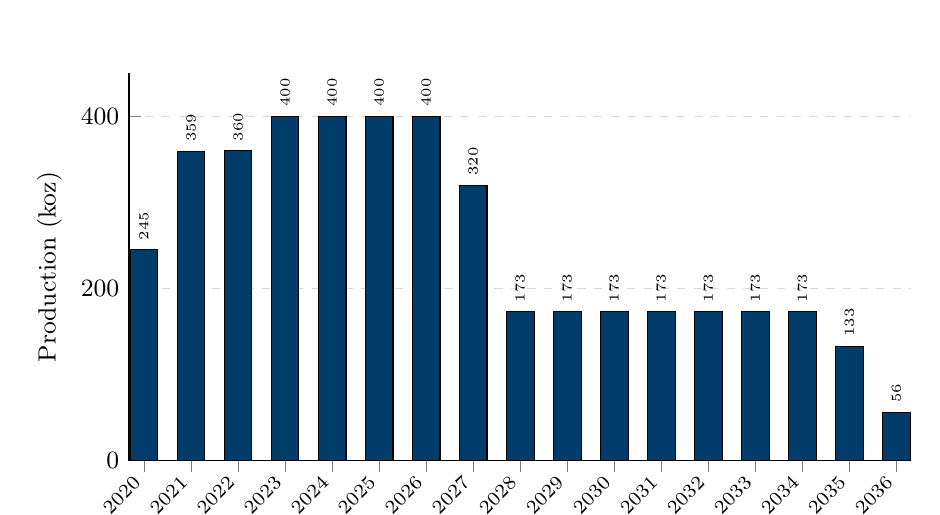
\begin{tikzpicture}
\begin{axis}[
  width=0.95\textwidth, height=6.5cm,
  ybar, bar width=10pt,
  symbolic x coords={2020,2021,2022,2023,2024,2025,2026,2027,2028,2029,2030,2031,2032,2033,2034,2035,2036},
  xtick=data, x tick label style={rotate=45,anchor=east,font=\scriptsize},
  ylabel={Production (koz)}, ymin=0, ymax=450,
  ylabel style={font=\small}, tick label style={font=\small},
  enlarge x limits=0.02,
  axis lines*=left,
  ymajorgrids, grid style={dashed,gray!30},
  bar shift=0pt,
  nodes near coords, every node near coord/.append style={font=\tiny, rotate=90, anchor=west},
]
\addplot[fill=itieblue] coordinates {
 (2020,245)(2021,359)(2022,360)(2023,400)(2024,400)(2025,400)(2026,400)
 (2027,320)(2028,173)(2029,173)(2030,173)(2031,173)(2032,173)(2033,173)
 (2034,173)(2035,133)(2036,56)
};
\end{axis}
\end{tikzpicture}
\caption{Profil de production aurifère de Sabodala-Massawa, 2020-2036 (milliers d'onces)}
\label{fig:production}
\end{figure}

\subsection{Dépenses d'investissement}

Les dépenses d'investissement de développement (colonne « \CAPEX{} développement » du tableau~\ref{tab:profil-production}) correspondent à la ligne « \emph{Total Development} » du tableau de synthèse des coûts en capital du PFS, qui regroupe les phases~1 et~2 de mise à niveau de l'usine Massawa, le développement souterrain et la relocalisation de communautés. Les dépenses de maintien en exploitation (\emph{sustaining capital}) correspondent à la ligne « \emph{Sustaining Capex} » du tableau de synthèse des flux de trésorerie. Aucune dépense d'exploration n'est intégrée au profil, conformément au périmètre de l'analyse économique du PFS, qui exclut les coûts d'exploration de l'estimation des flux de trésorerie.

\subsection{Coûts d'exploitation}

Le modèle NRGI ne comporte, dans sa feuille de calcul, qu'une seule ligne de coût d'exploitation unitaire (exprimée en \$US par once), les lignes complémentaires prévues dans la feuille de paramètres (broyage, autres, énergie, services domestiques) n'étant pas reprises dans les formules de calcul du flux de trésorerie. Pour ne pas modifier la structure de calcul du classeur --- conformément à la contrainte de préservation de l'intégrité méthodologique de l'outil --- l'ensemble des coûts d'exploitation du PFS (exploitation minière à ciel ouvert et souterraine, traitement WOL et ROT, coûts généraux et administratifs, administration régionale) a été agrégé en un coût unitaire annuel, calculé comme~:
\begin{equation}
  c_t = \frac{C^{\text{OP}}_t + C^{\text{UG}}_t + C^{\text{WOL}}_t + C^{\text{ROT}}_t + C^{\text{G\&A}}_t + C^{\text{adm.~rég.}}_t}{Q_t}
\end{equation}
où $Q_t$ est la production annuelle en onces et chaque terme $C_t$ le coût annuel correspondant, exprimé en millions \$US, issu des tableaux de synthèse des coûts d'exploitation du PFS. Cette agrégation explique le profil en dents de scie du coût unitaire observé dans le tableau~\ref{tab:profil-production}~: les années 2028 à 2032, où la production chute fortement alors que les coûts fixes (administration, maintenance de l'usine ROT) restent élevés, affichent un coût unitaire proche de 900~\$US/oz, contre 450 à 550~\$US/oz pendant la période de production maximale.

\subsection{Prix de l'or et coûts de fermeture}

Le prix de l'or retenu (1\,600~\$US/once) correspond au cas central de l'analyse économique du PFS et a été reporté à la fois dans le paramètre de prix de référence et dans le paramètre de prix utilisé pour le calcul de l'impôt sur les profits excédentaires (où il se substitue au prix de 1\,300~\$US/once du profil générique d'origine~; le prix de réserve, utilisé par certains régimes pour la définition de seuils, a été fixé à 1\,250~\$US/once conformément à l'hypothèse de réserve du PFS). Un coût de fermeture et de réhabilitation de 5~millions \$US a été affecté à la dernière année de production (2036), conformément à l'indication du PFS selon laquelle la majeure partie de ces coûts est engagée en fin de vie de mine.

\section{Construction du scénario fiscal « Sénégal »}
\label{sec:scenario-senegal}

La onzième colonne du tableau comparatif des régimes fiscaux --- vide dans la version d'origine, mais déjà référencée par l'ensemble des formules de calcul (plages de type \texttt{INDEX(H\textit{ligne}:R\textit{ligne}, \$F\$6)}) et par le sélecteur de régime --- a été renseignée avec les paramètres du régime sénégalais décrits à la section~\ref{sec:regime-sgo}. Le tableau~\ref{tab:regimes} reproduit, pour les quatre instruments fiscaux les plus déterminants, les paramètres retenus pour le Sénégal et pour les dix régimes de comparaison déjà présents dans l'outil.

\begin{table}[H]
\centering
\caption{Paramètres des principaux instruments fiscaux par régime}
\label{tab:regimes}
\small
\begin{tabular}{lcccc}
\toprule
Régime & Redevance & Impôt sur les & Participation & Droits de \\
       & (assiette) & bénéfices & gratuite de l'État & douane \\
\midrule
RDC -- 2002            & 2,5\,\% (nette) & 30,0\,\% & 5\,\%  & 5,0\,\% \\
RDC -- amendée (2018)  & 3,5\,\% (brute) & 35,0\,\% & 10\,\% & 5,0\,\% \\
Chili                  & 0\,\%           & 22,4\,\% & 0\,\%  & 0\,\% \\
Pérou                  & 0\,\%           & 28,0\,\% & 0\,\%  & 0\,\% \\
Australie-Occidentale  & 2,5\,\% (brute) & 30,0\,\% & 0\,\%  & 0\,\% \\
Tanzanie               & 4,0\,\% (brute) & 30,0\,\% & 0\,\%  & 0\,\% \\
Ghana                  & 5,0\,\% (brute) & 35,0\,\% & 10\,\% & 0\,\% \\
Zambie -- 2016         & 5,0\,\% (brute) & 30,0\,\% & 0\,\%  & 0\,\% \\
RDC -- redevance variable & 2,5\,\% (brute) & 30,0\,\% & 5\,\% & 5,0\,\% \\
RDC -- taxe sur la rente  & 2,5\,\% (brute) & 30,0\,\% & 5\,\% & 5,0\,\% \\
\textbf{Sénégal (SGO)} & \textbf{5,0\,\% (brute)} & \textbf{25,0\,\%} & \textbf{10\,\%} & \textbf{0,0\,\%} \\
\bottomrule
\end{tabular}

\vspace{0.2cm}
\footnotesize Source~: dix premiers régimes -- paramétrage d'origine de l'outil NRGI~; régime « Sénégal » -- construit par les auteurs d'après \citet{lycopodium2020pfs}, section~22.3-22.4 et \citet{senegal2016codeminier}.
\end{table}

Les autres paramètres du régime sénégalais --- modalités d'amortissement, report des pertes, taux de retenue à la source sur les dividendes --- n'étant pas détaillés dans le PFS, ils ont été repris, à titre conservatoire, des valeurs du régime « RDC amendée », régime le plus proche du Sénégal en termes de taux d'imposition global sur les bénéfices avant l'amendement de 2018. Cette convention n'affecte que marginalement les résultats présentés au chapitre~\ref{chap:resultats}, dans la mesure où, pour le profil de Sabodala-Massawa --- dont le flux de trésorerie avant impôt est positif dès la première année --- ni le report de pertes ni le calendrier d'amortissement ne deviennent contraignants.

Le sélecteur de régime de l'outil (paramètre \texttt{F6}) reste positionné, par défaut, sur le régime « RDC amendée », ce qui permet de continuer à utiliser l'outil pour son objet initial (analyse du code minier congolais)~; il suffit de le repositionner sur la valeur~11 pour activer le régime « Sénégal » et obtenir directement, pour le profil Sabodala-Massawa, les résultats détaillés présentés au chapitre~\ref{chap:resultats}.

\section{Hypothèses économiques et financières générales, et limites}

Les hypothèses économiques et financières générales du modèle --- taux d'actualisation de l'État (10\,\%) et de l'investisseur (12,5\,\%), taux d'inflation du dollar (2\,\%), part de l'investissement financée par emprunt (50\,\%), durée de remboursement (5~ans) et taux d'intérêt réel (12,5\,\%) --- correspondent aux valeurs de référence du modèle FARI et n'ont pas été modifiées, le PFS de Sabodala-Massawa ne fournissant pas d'hypothèses de financement alternatives explicites pour cette extension de mine déjà en exploitation.

Trois limites méritent d'être signalées à ce stade~:
\begin{enumerate}
  \item le modèle ne représente que les instruments fiscaux génériques (redevance, impôt sur les bénéfices, participation de l'État, retenue à la source, droits de douane, instruments progressifs)~; les flux spécifiques à la transaction Massawa (paiement initial de 15~millions \$US, \emph{gold stream} Franco-Nevada) n'y figurent pas, pour les raisons indiquées à la section~\ref{sec:regime-sgo}~;
  \item le profil de Sabodala-Massawa correspond à l'\textbf{extension} d'une mine déjà en production, et non à un projet \emph{greenfield}~: le flux de trésorerie avant impôt est positif dès la première année du modèle (2020), ce qui prive de sens les indicateurs de \TRI{} et de période de récupération calculés par l'outil --- conçus pour un projet dont les premières années sont marquées par un investissement net négatif. Ce point est discuté en détail à la section~\ref{sec:limites-tri}~;
  \item enfin, le modèle suppose, conformément à la méthodologie FARI, un prix de l'or constant en termes réels sur toute la période~; aucune analyse de sensibilité au prix n'est présentée dans ce rapport, le PFS lui-même limitant cette sensibilité à quatre scénarios de prix (1\,500 à 1\,800~\$US/once) appliqués à la \VAN{} globale du projet et non à sa décomposition par instrument fiscal.
\end{enumerate}

\chapter{Résultats et analyse}
\label{chap:resultats}

Ce chapitre présente les résultats obtenus en appliquant le modèle décrit au chapitre~\ref{chap:methodo} au profil opérationnel de Sabodala-Massawa. Sauf indication contraire, les montants sont exprimés en millions de dollars US constants (« réels »), cumulés sur la durée de vie du projet (2020-2036), conformément à la présentation retenue par l'outil NRGI dans sa feuille de résultats.

\section{Flux de trésorerie du projet et partage entre l'État et l'investisseur}

Le flux de trésorerie du projet avant toute imposition --- c'est-à-dire la différence entre le chiffre d'affaires et la somme des dépenses d'investissement, des coûts d'exploitation et des coûts de fermeture --- atteint 3\,595,4~millions \$US sur l'ensemble de la période, pour une valeur actuelle nette de 2\,122,7~millions \$US au taux d'actualisation de 10\,\%. Ce montant ne dépend pas du régime fiscal retenu~: il représente la « taille du gâteau » à partager entre l'État, l'investisseur et, le cas échéant, les créanciers.

Le tableau~\ref{tab:repartition} présente la répartition de ce flux entre l'État et l'investisseur sous deux régimes~: le régime « RDC amendée », qui demeure le régime actif par défaut de l'outil, et le régime « Sénégal » construit pour ce rapport. Sous le régime sénégalais, l'État perçoit 1\,589,7~millions \$US, soit 44,3\,\% du flux avant impôt, contre 2\,072,8~millions \$US (57,6\,\%) sous le régime congolais amendé --- un écart de 483~millions \$US sur la durée de vie du projet, qui revient symétriquement à l'investisseur.

\begin{table}[H]
\centering
\caption{Répartition du flux de trésorerie avant impôt entre l'État et l'investisseur, par régime (millions \$US réels, cumul 2020-2036)}
\label{tab:repartition}
\begin{tabular}{lccc}
\toprule
 & RDC -- amendée & Sénégal (SGO) & Écart \\
\midrule
Recettes de l'État          & 2\,072,8 & 1\,589,7 & $-$483,0 \\
Flux de l'investisseur après impôt & 1\,522,6 & 2\,005,6 & $+$483,0 \\
\midrule
Flux total avant impôt      & \multicolumn{2}{c}{3\,595,4} & -- \\
\TEMI                        & 57,6\,\% & 44,3\,\% & $-$13,3 points \\
\bottomrule
\end{tabular}
\end{table}

Cet écart de 13,3 points de \TEMI{} s'explique principalement par deux différences de paramétrage~: d'une part, le taux d'impôt sur les bénéfices, plus faible au Sénégal (25\,\% contre 35\,\%)~; d'autre part, l'exonération de droits de douane dont bénéficie SGO au titre de son statut d'entreprise franche d'exportation, qui n'a pas d'équivalent dans le régime congolais amendé (droits de douane de 5\,\%). À l'inverse, la redevance --- plus élevée au Sénégal (5\,\% contre 3,5\,\%, sur une assiette brute dans les deux cas) --- et la participation gratuite de l'État --- identique (10\,\%) --- jouent en sens inverse, mais de façon insuffisante pour compenser les deux premiers effets.

\section{Structure des recettes publiques par instrument fiscal}

Le tableau~\ref{tab:instruments} et la figure~\ref{fig:instruments} détaillent la composition des recettes de l'État pour les deux régimes, par instrument fiscal.

\begin{table}[H]
\centering
\caption{Recettes de l'État par instrument fiscal (millions \$US réels, cumul 2020-2036)}
\label{tab:instruments}
\small
\begin{tabular}{lrrrr}
\toprule
Instrument fiscal & \multicolumn{2}{c}{RDC -- amendée} & \multicolumn{2}{c}{Sénégal (SGO)} \\
 & Montant & Part & Montant & Part \\
\midrule
Bonus de signature                       & 0,0     & 0,0\,\%  & 0,0     & 0,0\,\%  \\
Droits de douane                         & 129,7   & 6,3\,\%  & 0,0     & 0,0\,\%  \\
Redevance                                & 239,9   & 11,6\,\% & 342,7   & 21,6\,\% \\
Impôt sur les bénéfices                  & 1\,121,1 & 54,1\,\% & 776,6  & 48,8\,\% \\
Impôt sur les profits excédentaires      & 224,9   & 10,9\,\% & 0,0     & 0,0\,\%  \\
Participation gratuite de l'État         & 188,0   & 9,1\,\%  & 247,6   & 15,6\,\% \\
Prélèvement à la source sur dividendes   & 169,2   & 8,2\,\%  & 222,8   & 14,0\,\% \\
\midrule
\textbf{Total} & \textbf{2\,072,8} & \textbf{100,0\,\%} & \textbf{1\,589,7} & \textbf{100,0\,\%} \\
\bottomrule
\end{tabular}

\vspace{0.2cm}
\footnotesize Les instruments « taxe provinciale », « redevance à taux variable sur les prix », « impôt sur la marge opérationnelle », « impôt sur la rente » et « impôt sur les bénéfices à taux variable » sont nuls dans les deux régimes et n'ont pas été reproduits dans le tableau.
\end{table}

\begin{figure}[H]
\centering
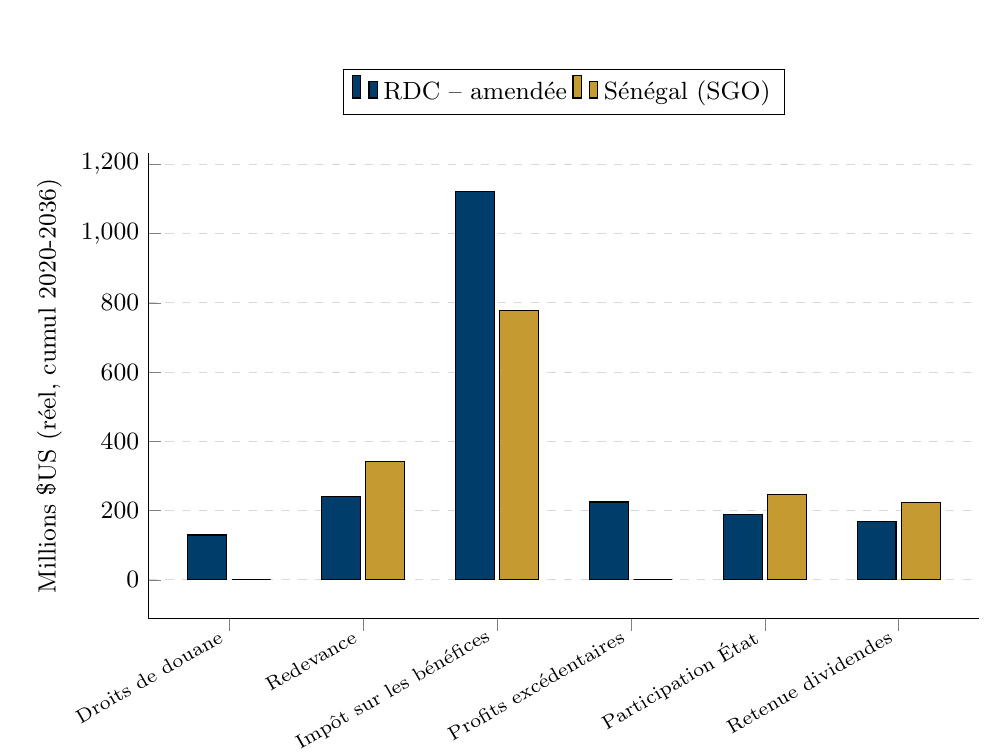
\begin{tikzpicture}
\begin{axis}[
  width=\textwidth, height=7.5cm,
  ybar, bar width=14pt,
  symbolic x coords={Droits de douane,Redevance,Impôt sur les bénéfices,Profits excédentaires,Participation État,Retenue dividendes},
  xtick=data, x tick label style={rotate=30,anchor=east,font=\scriptsize},
  ylabel={Millions \$US (réel, cumul 2020-2036)},
  ylabel style={font=\small}, tick label style={font=\small},
  enlarge x limits=0.12,
  legend style={at={(0.5,1.08)},anchor=south,legend columns=-1,font=\small},
  ymajorgrids, grid style={dashed,gray!30},
  axis lines*=left,
]
\addplot[fill=itieblue] coordinates {
 (Droits de douane,129.7)(Redevance,239.9)(Impôt sur les bénéfices,1121.1)
 (Profits excédentaires,224.9)(Participation État,188.0)(Retenue dividendes,169.2)
};
\addplot[fill=itiegold] coordinates {
 (Droits de douane,0)(Redevance,342.7)(Impôt sur les bénéfices,776.6)
 (Profits excédentaires,0)(Participation État,247.6)(Retenue dividendes,222.8)
};
\legend{RDC -- amendée, Sénégal (SGO)}
\end{axis}
\end{tikzpicture}
\caption{Recettes de l'État par instrument fiscal -- comparaison RDC amendée / Sénégal}
\label{fig:instruments}
\end{figure}

Trois enseignements se dégagent de cette comparaison. Premièrement, l'impôt sur les bénéfices demeure, dans les deux régimes, la principale source de recettes (49 à 54\,\% du total), ce qui confirme la sensibilité des recettes publiques à la profitabilité du projet --- donc au prix de l'or --- plutôt qu'à un instrument assis sur le volume. Deuxièmement, l'absence de droits de douane et d'impôt sur les profits excédentaires dans le régime sénégalais --- soit 17,2\,\% des recettes du régime congolais amendé --- n'est que partiellement compensée par le supplément de redevance (+102,8~millions \$US) et de participation de l'État (+59,6~millions \$US). Troisièmement, la retenue à la source sur les dividendes, dont le poids relatif passe de 8,2\,\% à 14,0\,\%, illustre le fait qu'une part accrue des recettes publiques sénégalaises est conditionnée à la distribution effective de dividendes par SGO --- recettes par construction plus tardives et plus incertaines que celles tirées de la redevance ou de l'impôt sur les bénéfices, qui sont prélevées dès que le projet est en exploitation et profitable, respectivement.

\section{Le \TEMI{} sénégalais dans la comparaison internationale}

La figure~\ref{fig:temi} et le tableau~\ref{tab:temi} positionnent le \TEMI{} obtenu pour le régime sénégalais --- 44,3\,\% --- parmi les dix régimes de comparaison déjà intégrés dans l'outil NRGI, tous appliqués au même profil de production que celui de Sabodala-Massawa. Cette mise en perspective permet d'apprécier, à profil opérationnel identique, l'effet du seul paramétrage fiscal sur le partage de la rente.

\begin{table}[H]
\centering
\caption{\TEMI{} par régime fiscal, appliqué au profil de production de Sabodala-Massawa}
\label{tab:temi}
\begin{tabular}{lc}
\toprule
Régime & \TEMI \\
\midrule
RDC -- amendée (2018)            & 57,6\,\% \\
Australie-Occidentale            & 54,7\,\% \\
Chili                             & 53,4\,\% \\
Ghana                             & 50,2\,\% \\
RDC -- taxe sur la rente         & 50,7\,\% \\
RDC -- redevance à taux variable & 44,8\,\% \\
\textbf{Sénégal (SGO)}           & \textbf{44,3\,\%} \\
RDC -- 2002                      & 44,5\,\% \\
Zambie -- 2016                   & 42,9\,\% \\
Tanzanie                         & 40,2\,\% \\
Pérou                             & 37,9\,\% \\
\bottomrule
\end{tabular}
\end{table}

\begin{figure}[H]
\centering
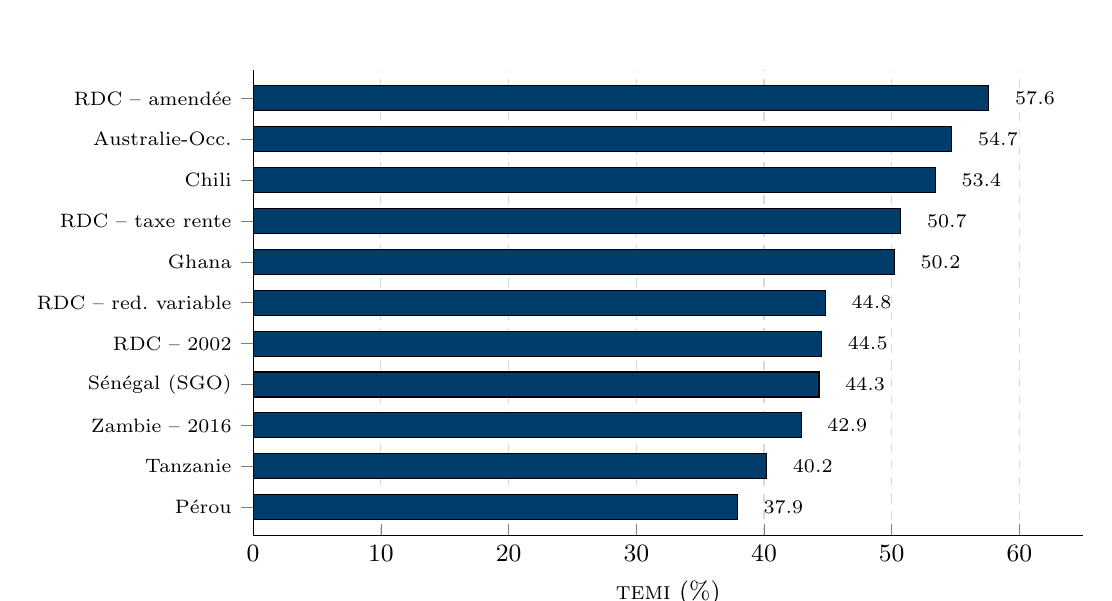
\begin{tikzpicture}
\begin{axis}[
  width=\textwidth, height=7.5cm,
  xbar, bar width=9pt,
  symbolic y coords={Pérou,Tanzanie,Zambie -- 2016,{Sénégal (SGO)},RDC -- 2002,{RDC -- red. variable},Ghana,{RDC -- taxe rente},Chili,{Australie-Occ.},{RDC -- amendée}},
  ytick=data, y tick label style={font=\scriptsize},
  xlabel={\TEMI{} (\%)}, xmin=0, xmax=65,
  xlabel style={font=\small}, tick label style={font=\small},
  enlarge y limits=0.07,
  xmajorgrids, grid style={dashed,gray!30},
  axis lines*=left,
  nodes near coords={\pgfmathprintnumber[fixed,fixed zerofill,precision=1]{\pgfplotspointmeta}},
  every node near coord/.append style={font=\scriptsize, xshift=6pt},
]
\addplot[fill=itieblue] coordinates {
 (37.9,Pérou)
 (40.2,Tanzanie)
 (42.9,Zambie -- 2016)
 (44.3,{Sénégal (SGO)})
 (44.5,RDC -- 2002)
 (44.8,{RDC -- red. variable})
 (50.2,Ghana)
 (50.7,{RDC -- taxe rente})
 (53.4,Chili)
 (54.7,{Australie-Occ.})
 (57.6,{RDC -- amendée})
};
\end{axis}
\end{tikzpicture}
\caption{Comparaison internationale du \TEMI{}, profil de production Sabodala-Massawa (le Sénégal est représenté en quatrième position à partir du bas)}
\label{fig:temi}
\end{figure}

Le \TEMI{} sénégalais se situe ainsi dans la partie inférieure de la distribution des onze régimes comparés, à un niveau quasiment identique à celui du code minier congolais de 2002 (avant l'amendement de 2018) et au régime congolais à redevance variable, mais nettement inférieur à celui du code minier congolais amendé, du régime australien et du régime chilien --- pourtant souvent cités comme exemples de régimes compétitifs pour les pays développés. Deux régimes seulement --- la Tanzanie et le Pérou --- présentent un \TEMI{} inférieur à celui du Sénégal pour ce profil de projet. Cette position relativement basse dans la comparaison internationale doit cependant être interprétée à la lumière de la remarque formulée au chapitre~\ref{chap:methodo}~: le régime sénégalais modélisé ne couvre pas les flux additionnels liés à la transaction Massawa (paiement initial et \emph{gold stream}), qui --- bien que de nature contractuelle et non fiscale --- représentent, sur la durée du PFS, un ordre de grandeur de 155~millions \$US (15~millions \$US de paiement initial et environ 140~millions \$US de valeur actualisée du \emph{gold stream}), soit près de 10\,\% des recettes fiscales calculées par le modèle pour le régime sénégalais. Leur prise en compte rapprocherait le \TEMI{} effectif de SGO du niveau observé pour le régime congolais à taxe sur la rente ou pour le Ghana.

\section{Limites de l'approche pour un projet d'extension de mine}
\label{sec:limites-tri}

Les indicateurs de rentabilité du point de vue de l'investisseur calculés par l'outil --- \TRI{} avant et après impôt, période de récupération actualisée et non actualisée --- renvoient tous une valeur nulle, quel que soit le régime fiscal retenu (tableau~\ref{tab:tri}).

\begin{table}[H]
\centering
\caption{Indicateurs de rentabilité calculés par le modèle}
\label{tab:tri}
\begin{tabular}{lc}
\toprule
Indicateur & Valeur \\
\midrule
\VAN{} avant impôt (actualisée à 10\,\%) & 2\,122,7 millions \$US \\
\TRI{} avant impôt & non défini (0 affiché) \\
\TRI{} après impôt & non défini (0 affiché) \\
Période de récupération (non actualisée) & non définie (0 affiché) \\
Période de récupération (actualisée) & non définie (0 affiché) \\
\bottomrule
\end{tabular}
\end{table}

Cette absence de résultat n'est pas une erreur de calcul, mais la conséquence directe de la nature du profil de Sabodala-Massawa~: le flux de trésorerie avant impôt de la première année du modèle (2020) est déjà positif (143,0~millions \$US), et il le reste pour chacune des dix-sept années du projet. Or, par construction, le \TRI{} d'une série de flux de trésorerie n'existe que si cette série change au moins une fois de signe~: la fonction financière utilisée par le modèle ne trouve donc aucune racine et renvoie une erreur, que la formule convertit par défaut en zéro. La période de récupération de l'investissement --- définie comme le nombre d'années nécessaire pour que le cumul des flux de trésorerie actualisés devienne positif --- est, pour la même raison, immédiatement atteinte (dès l'année~0) et n'est donc pas non plus interprétable comme un indicateur de risque.

Cette situation est caractéristique des outils FARI/NRGI, conçus à l'origine pour des projets \emph{greenfield}, dont la phase de construction se traduit par plusieurs années de flux négatifs avant le démarrage de la production. Sabodala-Massawa, en tant qu'\textbf{extension} d'une mine déjà en exploitation --- où les dépenses d'investissement de la phase~1 de Massawa (160~millions \$US en 2022, soit la plus importante annuité du profil) sont financées par les flux de trésorerie dégagés par les opérations existantes --- ne présente, à l'échelle du modèle, aucune année de flux net négatif.

Cette limite n'invalide pas pour autant les résultats présentés aux sections précédentes~: la \VAN{} et le \TEMI, qui ne reposent pas sur une condition de changement de signe, restent parfaitement définis et interprétables. Elle invite néanmoins à la prudence quant à l'utilisation de ce type d'outil pour les décisions d'investissement relatives à des projets d'extension~: un investisseur ou une administration souhaitant évaluer la rentabilité \emph{marginale} de la décision d'investissement (ici, la mise en valeur du gisement Massawa) devrait isoler, dans le flux de trésorerie, la seule part additionnelle liée à cette décision --- ce qui sortirait du cadre du présent exercice, fondé sur le profil consolidé du complexe Sabodala-Massawa tel que présenté dans le PFS.

%\chapter{Implications pour le suivi de la fiscalité minière par l'ITIE Sénégal}
\label{chap:recommandations}

L'exercice présenté dans ce rapport, bien que limité à un seul projet et à un seul régime fiscal, met en évidence l'intérêt d'un outil de simulation de type FARI/NRGI pour le travail de l'ITIE Sénégal~: il permet de transformer des paramètres contractuels --- taux de redevance, taux d'impôt, quotités de participation --- en un indicateur de synthèse (\TEMI) directement comparable à celui d'autres juridictions, et de décomposer les recettes attendues par instrument fiscal sur la durée de vie d'un projet. Cette section propose quelques pistes pour l'appropriation de cette démarche par le Comité National ITIE Sénégal, organisées en trois axes~: la consolidation des données d'entrée, le suivi dans le temps, et la transparence sur les arrangements contractuels particuliers.

\section{Consolider les données d'entrée nécessaires à la modélisation}

L'application du modèle à Sabodala-Massawa a mobilisé des données --- calendrier de production, structure des coûts, paramètres fiscaux --- dispersées dans un document technique de plusieurs centaines de pages (le PFS), rédigé en anglais et destiné en premier lieu aux investisseurs et aux marchés financiers. Une première recommandation consiste donc à établir, pour chaque titre minier en phase d'exploitation, une fiche de synthèse normalisée reprenant ces paramètres dans un format directement exploitable par un outil de simulation~: calendrier de production prévisionnel, dépenses d'investissement de développement et de maintien, structure des coûts d'exploitation, et paramètres effectifs du régime fiscal applicable --- en distinguant explicitement les dispositions de droit commun et celles résultant d'une convention particulière. La constitution progressive d'une telle base, pour l'ensemble des titres en exploitation (or, zircon, phosphates, attapulgite), permettrait de reproduire l'exercice réalisé ici pour Sabodala-Massawa à l'échelle du secteur extractif sénégalais dans son ensemble, et de disposer d'une estimation \emph{ex ante} des recettes attendues à comparer aux recettes effectivement déclarées dans les rapports de conciliation.

\section{Assurer un suivi dans le temps du \TEMI{} et de ses déterminants}

Le \TEMI{} calculé dans ce rapport (44,3\,\%) constitue une photographie à un instant donné, fondée sur un prix de l'or de 1\,600~\$US/once et sur le calendrier de production du PFS de 2020. Or, le \TEMI{} d'un projet minier varie avec le prix de la ressource --- principalement via la part relative de l'impôt sur les bénéfices, qui croît plus que proportionnellement avec la profitabilité --- ainsi qu'avec l'arrivée à échéance de certaines exonérations temporaires (TVA, statut d'entreprise franche). Un suivi périodique --- par exemple annuel, à l'occasion de la mise à jour des rapports de conciliation --- de ce \TEMI{}, recalculé sur la base des paramètres de production et de prix effectivement observés, permettrait à l'ITIE Sénégal de documenter l'évolution de la part de la rente minière captée par l'État au fil du cycle de prix des matières premières, et de objectiver le débat --- récurrent dans la plupart des juridictions minières --- sur le caractère « équitable » ou non du partage de cette rente.

\section{Documenter les arrangements contractuels qui échappent au régime fiscal général}

L'écart, souligné au chapitre~\ref{chap:resultats}, entre le \TEMI{} calculé pour le seul régime fiscal général applicable à SGO (44,3\,\%) et l'ordre de grandeur des flux additionnels liés à la transaction Massawa (paiement initial et \emph{gold stream} Franco-Nevada, de l'ordre de 155~millions \$US sur la durée du PFS) illustre une limite plus générale des modèles de type FARI~: ils ne représentent que les instruments fiscaux et parafiscaux « généralisables », et non les arrangements financiers propres à une transaction donnée entre actionnaires privés, qui peuvent pourtant avoir une incidence significative sur la valeur captée localement par rapport à la valeur exportée. La Norme ITIE prévoit déjà la divulgation des contrats et conventions miniers~; ce travail suggère qu'une attention particulière devrait être portée, dans les rapports de conciliation et dans la documentation publiée par l'ITIE Sénégal, à l'identification et, dans la mesure du possible, à la quantification de ces flux contractuels additionnels (contrats de \emph{streaming} ou d'\emph{offtake}, options sur participations, paiements d'étape liés à des acquisitions d'actifs), afin de donner une image complète du partage de la valeur générée par un projet minier, au-delà du seul régime fiscal de droit commun.

\section{Capitaliser sur la onzième colonne ajoutée au modèle}

D'un point de vue pratique, l'ajout d'un onzième régime « Sénégal » au classeur NRGI --- réalisé en complétant une colonne de paramètres déjà prévue par la structure de l'outil, sans modification des formules existantes --- constitue une base directement réutilisable. Il suffit, pour analyser un autre projet minier sénégalais (zircon, phosphates, ou un autre projet aurifère), de répliquer la feuille de paramètres avec le profil opérationnel et les paramètres fiscaux propres à ce projet, le régime « Sénégal » pouvant être affiné --- par exemple en distinguant le régime de droit commun du code minier de 2016 (applicable aux nouveaux titres) du régime conventionnel applicable aux titres antérieurs comme Sabodala. À moyen terme, la constitution d'une bibliothèque de scénarios fiscaux sénégalais --- droit commun 2016, principales conventions minières en vigueur --- au sein d'un même outil permettrait à l'ITIE Sénégal de réaliser, pour tout nouveau projet en cours d'instruction, une comparaison rapide entre le régime envisagé dans la convention et le régime de droit commun, contribuant ainsi à objectiver les négociations entre l'État et les investisseurs évoquées au chapitre~\ref{chap:cadre}.

\chapter*{Conclusion}
\addcontentsline{toc}{chapter}{Conclusion}
\markboth{Conclusion}{}

Ce rapport a appliqué, pour la première fois à notre connaissance, l'outil de modélisation financière d'une mine d'or diffusé par NRGI --- adaptation simplifiée de la méthodologie FARI du FMI --- au cas du secteur aurifère sénégalais, en s'appuyant sur les données techniques et économiques de l'étude de préfaisabilité du projet Sabodala-Massawa publiée en 2020. Deux opérations ont été nécessaires~: remplacer le profil opérationnel générique de l'outil par le profil réel du projet (production, dépenses d'investissement, coûts d'exploitation, prix de l'or) sur la période 2020-2036, et compléter le tableau comparatif des régimes fiscaux --- qui comportait dix régimes pré-paramétrés et une colonne vide --- par un onzième régime reproduisant les paramètres effectivement applicables à Sabodala Gold Operations (redevance de 5\,\% sur la valeur des expéditions, impôt sur les sociétés de 25\,\%, participation gratuite de l'État de 10\,\%, exonération de droits de douane).

Les résultats indiquent que, pour ce profil de projet, le régime fiscal sénégalais génère un \TEMI{} de 44,3\,\%, sensiblement inférieur à celui du code minier congolais amendé (57,6\,\%) auquel l'outil était initialement consacré, et proche du bas de la distribution des onze régimes comparés --- seuls la Tanzanie et le Pérou présentant un \TEMI{} inférieur pour ce même profil. La structure des recettes publiques sénégalaises est dominée par l'impôt sur les bénéfices (49\,\%), suivi de la redevance (22\,\%), de la participation gratuite de l'État (16\,\%) et de la retenue à la source sur les dividendes (14\,\%)~; l'absence de droits de douane, liée au statut d'entreprise franche d'exportation de SGO, constitue l'écart le plus significatif avec les régimes de comparaison.

Un second résultat, de nature davantage méthodologique, concerne les indicateurs de rentabilité du point de vue de l'investisseur~: le \TRI{} avant et après impôt, ainsi que les périodes de récupération, ne sont pas interprétables pour Sabodala-Massawa, dans la mesure où le flux de trésorerie avant impôt du projet est positif dès la première année du modèle --- caractéristique d'un projet d'extension d'une mine déjà en production, et non d'un projet \emph{greenfield} pour lequel ces indicateurs ont été conçus. La \VAN{} et le \TEMI, en revanche, demeurent pleinement valides et constituent, à ce titre, les indicateurs les plus pertinents pour ce type de configuration.

Ces résultats appellent trois prolongements. D'une part, l'élargissement de l'exercice aux autres titres miniers en exploitation au Sénégal --- notamment dans le secteur du zircon et des phosphates --- permettrait de disposer d'une vue d'ensemble de la performance fiscale du secteur extractif, et non d'un seul projet. D'autre part, une analyse de sensibilité au prix de l'or, qui n'a pas été conduite ici par souci de cohérence avec le cas central retenu par le PFS, donnerait une mesure de la stabilité du \TEMI{} sénégalais sur le cycle des prix, complémentaire de la photographie statique présentée au chapitre~\ref{chap:resultats}. Enfin, la quantification --- même approximative --- des flux contractuels qui échappent au régime fiscal général, tels que le contrat d'approvisionnement en or conclu avec Franco-Nevada dans le cadre de l'acquisition de Massawa, permettrait de rapprocher le \TEMI{} « modélisé » du partage effectif de la valeur entre l'État sénégalais et les actionnaires du projet.

Au-delà de ces résultats propres à Sabodala-Massawa, ce rapport illustre la possibilité, pour une administration disposant de ressources d'analyse limitées, de s'appuyer sur des outils ouverts --- ici, le classeur NRGI --- pour produire des estimations chiffrées, reproductibles et actualisables de la performance fiscale d'un projet minier, sans remettre en cause l'intégrité méthodologique de ces outils. C'est dans cette perspective que les pistes formulées au chapitre~\ref{chap:recommandations} ont été proposées pour le travail futur du Comité National ITIE Sénégal.


% =========================================================
% BIBLIOGRAPHIE
% =========================================================
\clearpage
\bibliographystyle{apalike}
\bibliography{references}

% =========================================================
% ANNEXES
% =========================================================
\appendix
\chapter{Paramètres techniques complémentaires des régimes fiscaux comparés}
\label{annexe:a}

Le tableau~\ref{tab:regimes} (chapitre~\ref{chap:methodo}) présentait, pour les onze régimes comparés dans ce rapport, les paramètres relatifs à la redevance, à l'impôt sur les bénéfices, à la participation gratuite de l'État et aux droits de douane. Le tableau~\ref{tab:regimes-tech} ci-dessous complète cette présentation par les paramètres techniques relatifs au report des pertes, au régime d'amortissement et à la retenue à la source sur le revenu des valeurs mobilières (IRVM), ainsi que par les particularités propres à certains régimes.

\begin{table}[H]
\centering
\caption{Paramètres techniques complémentaires, par régime fiscal}
\label{tab:regimes-tech}
\footnotesize
\begin{tabular}{lcccp{4.7cm}}
\toprule
Régime & \makecell{Report des\\pertes (durée /\\limite annuelle)} & \makecell{Régime\\d'amortissement\\(années)} & IRVM & Particularités \\
\midrule
RDC -- 2002              & 5 ans / 100\,\% & 2  & 10,0\,\% & Amortissement accéléré (option activée) \\
RDC -- amendée (2018)    & 5 ans / 100\,\% & 5  & 10,0\,\% & Impôt sur les profits excédentaires~: 50\,\% au-delà d'un \TRI{} réel de 25\,\% \\
Chili                     & 100 ans / 100\,\% & 10 & 35,0\,\% & Taxe sur la marge opérationnelle (système~3) \\
Pérou                     & 4 ans / 100\,\%  & 10 & 6,8\,\%  & Taxe sur la marge opérationnelle (système~2) \\
Australie-Occidentale     & 100 ans / 100\,\% & 20 & 30,0\,\% & -- \\
Tanzanie                  & 100 ans / 100\,\% & 1  & 10,0\,\% & -- \\
Ghana                     & 5 ans / 100\,\%  & 5  & 8,0\,\%  & -- \\
Zambie -- 2016            & 10 ans / 50\,\%  & 4  & 10,0\,\% & -- \\
RDC -- redevance variable & 5 ans / 100\,\% & 5  & 10,0\,\% & Redevance à taux variable indexée sur le prix (système~4) \\
RDC -- taxe sur la rente  & 5 ans / 100\,\% & 5  & 10,0\,\% & Taxe sur la rente~: 7,5\,\% au-delà d'un seuil de \TRI{} réel de 25\,\% \\
\textbf{Sénégal (SGO)}    & 5 ans / 100\,\% & 5  & 10,0\,\% & Paramètres techniques non précisés par le PFS, repris du régime RDC amendée (voir section~\ref{sec:scenario-senegal}) \\
\bottomrule
\end{tabular}

\vspace{0.2cm}
\footnotesize Source~: paramétrage d'origine de l'outil NRGI pour les dix premiers régimes~; régime « Sénégal » construit par les auteurs.
\end{table}

\chapter{Traçabilité des données extraites du PFS de Sabodala-Massawa}
\label{annexe:b}

Le tableau~\ref{tab:tracabilite} récapitule, pour chacun des principaux paramètres insérés dans le modèle, la valeur retenue et la section ou le tableau du PFS \citep{lycopodium2020pfs} dont elle est issue, à des fins de traçabilité et de reproductibilité de l'exercice.

\begin{table}[H]
\centering
\caption{Correspondance entre les paramètres du modèle et les sources du PFS}
\label{tab:tracabilite}
\footnotesize
\begin{tabular}{p{4.3cm}p{2.6cm}p{6.8cm}}
\toprule
Paramètre du modèle & Valeur retenue & Source dans le PFS \\
\midrule
Réserves récupérables & 4\,284\,000 oz & Table~1.7 / Table~22.1 -- \emph{LOM Cash Flow Summary}, production totale récupérée \\
Calendrier de production (2020-2036) & cf. tableau~\ref{tab:profil-production} & Table~1.7 / Table~22.1, ligne \emph{Gold Produced} \\
\CAPEX{} de développement & 407~millions \$US (cumul) & Table~1.10 / Table~22.1, ligne \emph{Total Development} \\
Capital de maintien (\emph{sustaining}) & 253~millions \$US (cumul) & Table~22.1, ligne \emph{Sustaining Capex} \\
Coût opérationnel unitaire & cf. tableau~\ref{tab:profil-production} & Table~1.11 (synthèse des coûts d'exploitation) et Table~22.1 (administration régionale), agrégés selon l'équation de la section~\ref{sec:donnees-pfs} \\
Prix de l'or (cas central) & 1\,600~\$US/once & Table~1.12 / Table~22.1, hypothèse de prix retenue pour l'analyse économique \\
Prix de référence des réserves & 1\,250~\$US/once & Section~1.7, \emph{Mineral Reserves} \\
Coût de fermeture et réhabilitation & 5~millions \$US (en 2036) & Section~22.4.5, \emph{Closure} \\
Taux de redevance (régime Sénégal) & 5,0\,\% (assiette brute) & Section~22.3.1, \emph{Royalties} \\
Taux d'impôt sur les sociétés (régime Sénégal) & 25,0\,\% & Section~22.3.2, \emph{Corporate Income Tax} \\
Participation gratuite de l'État (régime Sénégal) & 10,0\,\% & Section~22.4.7, \emph{Minority Interest} \\
Droits de douane (régime Sénégal) & 0,0\,\% & Section~22.4.8, statut d'entreprise franche d'exportation \\
\bottomrule
\end{tabular}
\end{table}


\end{document}
